\chapter{Experiment Design}
\label{ch:experiment}
\paragraph{} This chapter describe the experiment we conducted using the system described in chapter~\ref{ch:system_design}. Section~\ref{sec:experimentdesign} shows the preliminary steps for preparing the system to our experiments, such as the selection of the input levels and the features. Section~\ref{sec:trainednets} shows the trained networks we used in our experiments and \ref{sec:experiments} describes the three experiment we set up in order to study the trained networks.

\section{Experiment setup}
\label{sec:experimentdesign}
\paragraph{} This section explains what choices have been made before training the models in order to conduct the experiments. In particular we had to select which data to use with the neural network given our technological constraints, the network input features and how to evaluate our approach.

\subsection{Input Levels Selection}
\label{sec:InputSelection}
\paragraph{} For preparing our experiments we filtered the DoomDataset by taking only the samples up to 128x128 in size and which had exactly 1 "floor". This led to a dataset of about 1000 samples, which are then augmented by rotation during the training process. This is motivated from the fact that even if the level orientation does not affect playability, using levels with more floors could lead the network to learn a correlation between floors (and how to arrange them inside the map) which could potentially be misleading or be just enforced by the sample size or the way the editor arranged them on the level coordinate space. Moreover, using only one-floor levels helped in reducing smaller artefacts that appeared as very small floors in resulting output.

\subsection{Feature Selection}
In selecting which numerical features $Y$ to use as network input we followed some assumption and criteria:
\begin{enumerate}
	\item \textit{Reconstructability:} In order to be able to analyse the resulting network, it is possible to use only features that can be reconstructed from the network output images with reasonable loss of information. For example, features what depends on the WAD representation of the level such as the number of sectors are too much dependant both on the editor used to build the level, and the algorithm we use to convert back images to WAD. On the contrary, features based on the Feature Maps are a better choice since they are evaluated using the same algorithm.
	\item \textit{Visibility:} In order to be selected as an input, a feature has to have a visual impact on the samples. While in principle neural networks can extract complex and possibly inscrutable structure in the data, we decided to use only features that can have a visual feedback on the Feature Maps.
	\item \textit{Robustness:} Other than having a visual impact on the samples, a good feature must be robust to noise in the feature maps, in other words it must not change greatly for small variation in the pixel colour the images. 
\end{enumerate}


\paragraph{} We selected a subset of features that reasonably satisfied these properties by comparing the feature values of a small number of visually different level sets. An example of level set and the corresponding values for the selected features is shown on figure~\ref{fig:feature_selection}. A summary of the feature we used in our experiment is:
\begin{itemize}
	\item \textit{level equivalent diameter}: Diameter of the circle having the same area as the level.
	\item \textit{level major axis length}: Length of the longest axis of the level, independent from the rotation.
	\item \textit{level minor axis length}: Length of the shortest axis of the level, independent from the rotation.
	\item \textit{level solidity}: Ratio between the area of the level and its convex hull. It's a metric of the level convexity.
	\item \textit{nodes (number of rooms)}: Count of the rooms in the room adjacency graph.
	\item \textit{distmap skewness}: Skewness of the distribution of each pixel distance from the closest wall. This metric is visually related to the balance between large and small areas.
	\item \textit{distmap kurtosis}: Kurtosis of the distribution of each pixel distance from the closest wall. This metric is visually related to the presence of both very large and very small areas, or area size variety.
\end{itemize}


 \begin{figure}[h!]
 	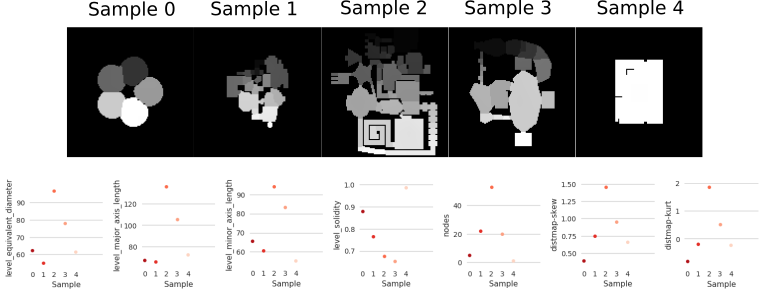
\includegraphics[width=\linewidth]{feature_selection.png}
 	\caption[Example of feature values]{Example of feature values on a set of 5 different levels. The first row shows the Room Map of the levels, in which each room is enumerated with a different grayscale colour. The second row shows the feature values for the features \textit{level equivalent diameter}, \textit{level major axis length}, \textit{level minor axis length}, \textit{level solidity}, \textit{nodes (number of rooms)}, \textit{distmap skewness} and \textit{distmap kurtosis}. }
 	\label{fig:feature_selection}
 \end{figure}

\subsection{Framework Evaluation}
\label{sec:modelevaluation}
\paragraph{} In order to evaluate the feasibility of our approach on the problem of level generation, we designed a set of experiments to test some of the settings that are possible to use with our framework. 
All the experiments involve comparing the distribution of true data and the one generated from the neural network, according to the features that is possible to calculate from the images generated from different models. In generating the models, we first trained a neural network without input features so that the generator is only controlled by the noise vector $Z$. We then added a set of features to our architecture and used it to train a network using the same random initialization. Details on the network we produced are shown in table~\ref{tab:trained_models}.

\newpage
\subsection{Trained Architectures}
\label{sec:trainednets}
\paragraph{} In training the models we kept fixed the WGAN-GP architecture, learning hyperparameters, the kernel size and the stride, while we varied the input features and the number of layers. During the development of the system we tried several different architectures and networks, but we show only the ones we conducted our experiments upon. For example, in our earlier experiments we tried using a single multi-valued map, but the results were affected from too much noise and artefacts. In the hope of obtaining better quality samples we also tried adding more layers to the network: although it showed to learn faster, it soon made the architecture unstable and the generator collapsed. Table~\ref{tab:trained_models} shows the final models we used in our experiments:

\begin{table}[h!]
	\begin{tabularx}{\textwidth}{| c | c | X | X | X | X |}
		\hline
		\textbf{Run Name} & \textbf{Iterations} & \textbf{Features} & \textbf{Maps} & \textbf{D Layers (filters)} & \textbf{G Layers (filters)} \\
		\hline
		
		
		
		unconditional & 36000 & 
		No features
		& 
		\begin{itemize}
			\raggedright
			\small
			\item[] floormap
			\item[] heightmap
			\item[] wallmap
			\item[] thingsmap
		\end{itemize}
		& 4 (1024, 512, 256, 128) & 4 (128, 256, 512, 1024)\\
		
		\hline
	
		conditional & 36000 & 
		\begin{itemize}
			\raggedright
			\small
			\item[] level equivalent diameter
			\item[] level major axis length
			\item[] level minor axis length
			\item[] level solidity
			\item[] nodes
			\item[] distmap-skew
			\item[] distmap-kurt
		\end{itemize}
		& 
		\begin{itemize}
			\raggedright
			\small
			\item[] floormap
			\item[] heightmap
			\item[] wallmap
			\item[] thingsmap
		\end{itemize}
		& 4 (1024, 512, 256, 128) & 4 (128, 256, 512, 1024)\\
		
		\hline
		
	\end{tabularx}
	\caption[ Trained Models ]{ Trained networks. }
	\label{tab:trained_models}
\end{table}	

\section{Experiments description}
\label{sec:experiments}
For assessing the capabilities of the networks we trained in relation to the problem of level generation we designed three experiments, which are described in the following paragraphs. Since the second experiment depends on the result of the first one, the results are showed together.

\subsection{Experiment 1: Unconditional generation}
In the first experiment we tested the ability of the "unconditional" network to generate levels that exhibit similar features to the original levels. 
For each level in the dataset we sampled one level from the unconditional network using random noise as input, we extracted the features from the generated level and we compared the distribution of the dataset with the distribution of the generated features. For comparing the true and generated feature distributions we used the \textit{Two-tailed Kolmogorov-Smirnov Statistical Test} \cite{KS-test} that utilizes a statistic calculated as the distance  between the empirical distribution functions of the two samples. The problem we solved with \textit{KS} can be resumed as: \\

\begin{equation}
	\begin{split}
	H_{0}:  & F_{G}(x) = F_{T}(x), \forall x \\
	H_{1}:  & F_{G}(x) \neq F_{T}(x), \text{for some x} \\
	\end{split}
\end{equation}

where $F_{G}(x)$ and $F_{T}(x)$ are the empirical distribution functions of the generated and true features, respectively. The tests have been corrected using the Bonferroni correction using a family-wise error rate (significance for the entire experiment) of 0.05; in correcting p-values we also considered the tests of experiment 2. Results are shown alongside the results of experiment 2 in tables \ref{tab:results-input-features} and \ref{tab:results-other-features}.

\subsection{Experiment 2: Addition of input features}
\label{sec:experiment-2}
In the second experiment we tested if the addition of features to the network input can have some effect on the generation of the samples. For doing this, we replicated the experiment one using the conditional network, then we compared the results with those obtained from the unconditional network. For each level in the dataset we sampled one level, using the true feature vector as input and
the same noise vectors used in experiment one. We then proceeded as in experiment one in testing the true and generated distributions of features. \\
For comparing the results of the unconditional and conditional networks we clustered the features in four groups, each one corresponding to a possible case: \\
\begin{enumerate}
	\item \textbf{F1:} Features for which the null hypothesis is rejected in both the unconditional and conditional networks. 
	\item \textbf{F2:} Features for which the null hypothesis is rejected for the unconditional network (experiment 1) but cannot be rejected for the conditional network. 
	\item \textbf{F3:} Features for which the null hypothesis cannot be rejected for both the unconditional  and conditional network.
	\item \textbf{F4:} Features for which the null hypothesis cannot be rejected for the unconditional network (experiment 1) but is rejected for the conditional network.
\end{enumerate}

Only for the features in the group F3, we also consider the distance (KS-stats) between the true and generated feature distributions in order to discover which network better reflects the feature distribution. This is reported as a "*" in the results tables \ref{tab:results-input-features} and \ref{tab:results-other-features}.

\subsection{Experiment 3: Controlling the generation}
In the third experiment we studied the impact of the input features on the generated levels from a qualitative point of view. In particular, we selected a set of levels from the dataset according to their feature values: for each input feature we selected the levels that match the 25th, 50th and 75th percentiles of the feature distribution, obtaining a total of $3 * \vert y_{i} \vert = 21$ levels. We then sampled 1000 levels from the conditioned network for each selected input feature vector, obtaining 1000 generated feature vectors for each input level. For each input feature, we plotted the three selected input values and the corresponding generated feature distributions, showing how the generated level distribution changes with respect to a change in the input feature. Results of this experiment are shown in figure~\ref{fig:results-exp3-features}.

\section{Summary}
\paragraph{} In this chapter we described the input selection for our trained models, consisting in levels up to 128 pixels and having one floor. We then described the general principles we used to select the input features for the conditional network, and lastly we proceeded to define our experiments. In the next chapter we show the results we obtained, while in the following one we discuss the results and present our conclusions.